\chapter{Конструкторский раздел}

В данном разделе будут спроектированы схемы алгоритмов.

\section{Схемы алгоритмов}

На вход алгоритмов подаются строки s1 и s2, а также их длины i и j соотетственно. На выходе единственное число - искомое расстояние.

На рисунке 2.1 представлена схема нерекурсивного алгоритма поиска расстояния Левенштейна с кэшем в форме двух строк.

На рисунке 2.2 представлена схема рекурсивного алгоритма поиска расстояния Левенштейна без кэша.

На рисунке 2.3 представлена схема рекурсивного алгоритма поиска расстояния Левенштейна с кэшем в форме матрицы. В данном алгоритме на вход также подается кэш с размерностью, так как алгоритм рекурсивный и по-другому кэш может быть утерян.

На рисунке 2.4 представлена схема рекурсивного алгоритма поиска расстояния Дамерау-Левенштейна без кэша.

\newpage 
\begin{figure}[H]
	\begin{center}
		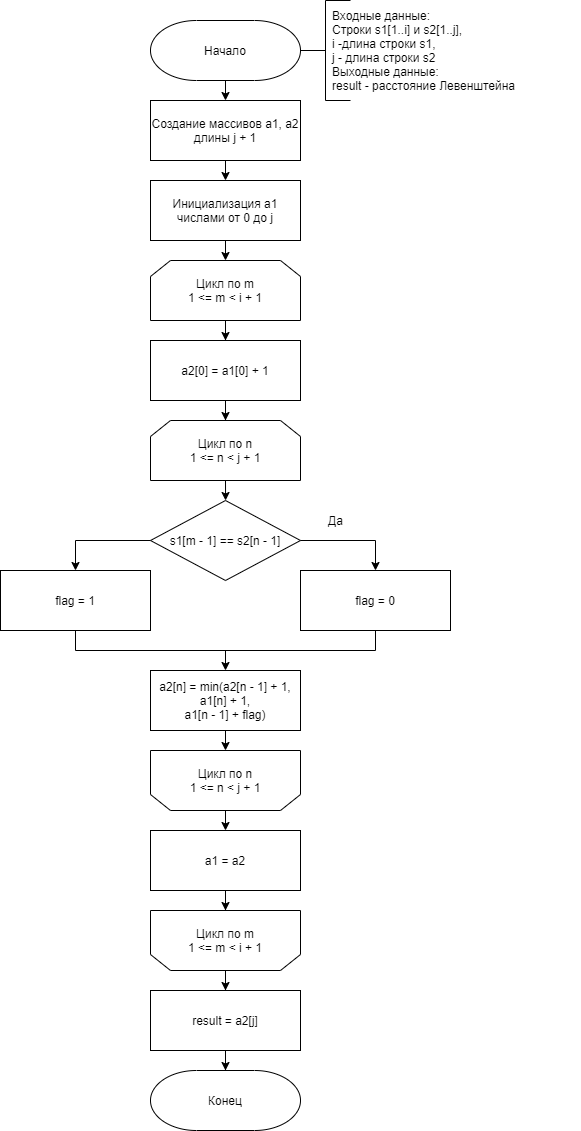
\includegraphics[scale=0.6]{assets/LevCacheTwoRows.png}
	\end{center}
	\caption{Схема нерекурсивного алгоритма поиска расстояния Левенштейна с кэшем в форме двух строк}
\end{figure}

\newpage 
\begin{figure}[H]
	\begin{center}
		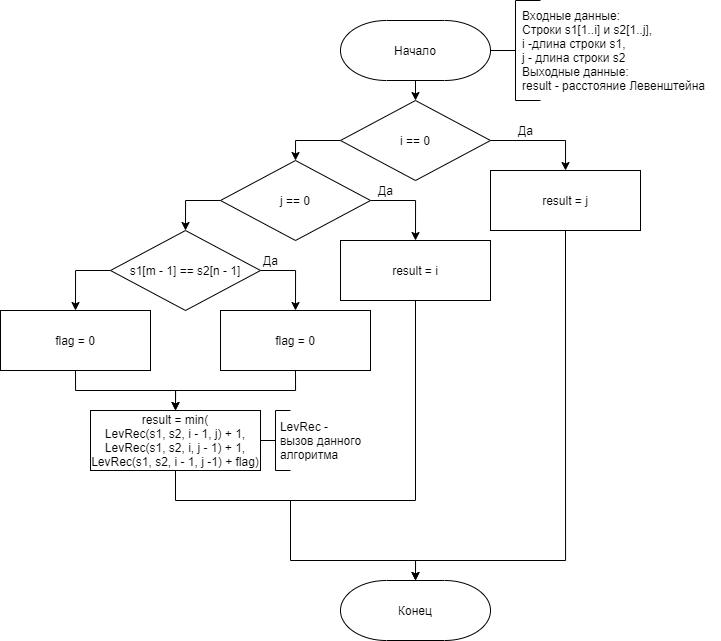
\includegraphics[scale=0.6]{assets/LevRecWithoutCache.png}
	\end{center}
	\caption{Схема рекурсивного алгоритма поиска расстояния Левенштейна без кэша}
\end{figure}

\newpage 
\begin{figure}[H]
	\begin{center}
		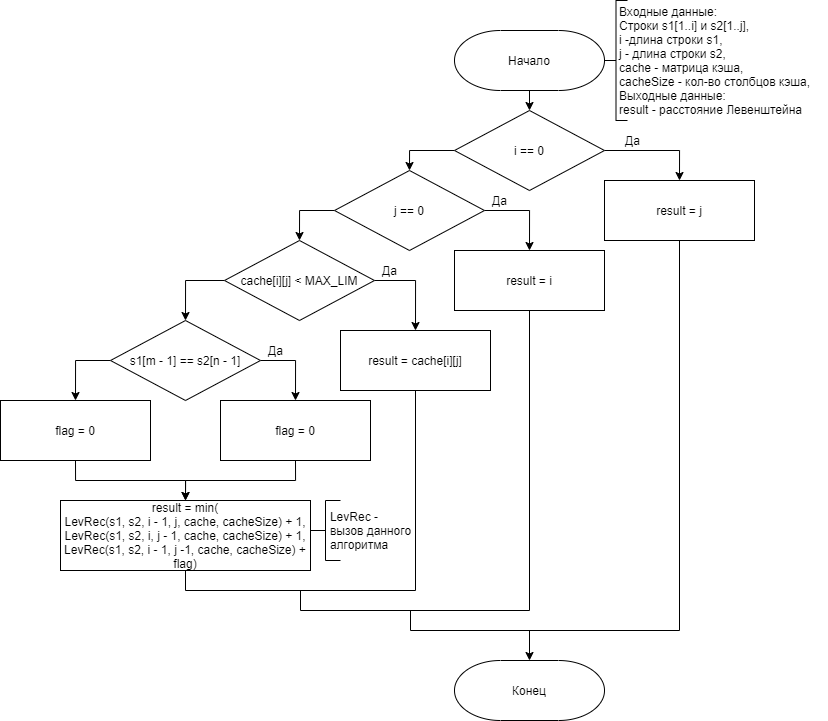
\includegraphics[scale=0.6]{assets/LevRecWithCache.png}
	\end{center}
	\caption{Схема рекурсивного алгоритма поиска расстояния Левенштейна с кэшем в форме матрицы}
\end{figure}

\newpage 
\begin{figure}[H]
	\begin{center}
		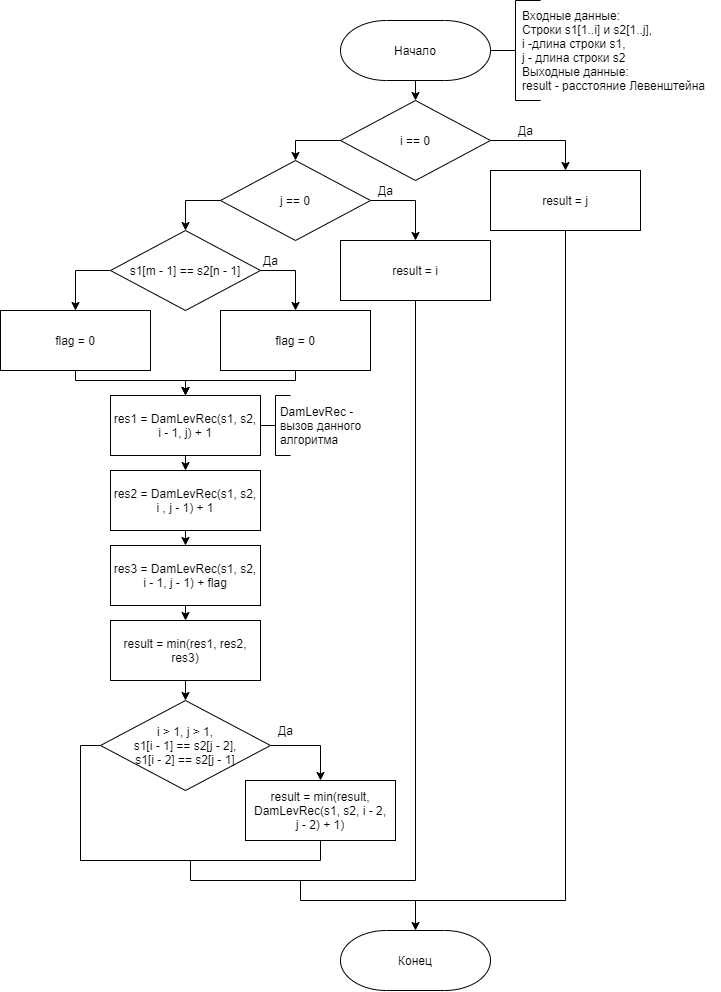
\includegraphics[scale=0.6]{assets/DamLevRecWithoutCache.png}
	\end{center}
	\caption{Схема рекурсивного алгоритма поиска расстояния Дамерау-Левенштейна без кэша}
\end{figure}

\section{Вывод}

На основе полученных в аналитическом разделе формул были спроектированы схемы алгоритмов.